%
% This is a borrowed LaTeX template file for lecture notes for CS267,
% Applications of Parallel Computing, UCBerkeley EECS Department.
%

\documentclass[twoside]{article}
\usepackage{titlesec}
\setlength{\oddsidemargin}{0.25 in}
\setlength{\evensidemargin}{-0.25 in}
\setlength{\topmargin}{-0.6 in}
\setlength{\textwidth}{6.5 in}
\setlength{\textheight}{8.5 in}
\setlength{\headsep}{0.75 in}
\setlength{\parindent}{0 in}
\setlength{\parskip}{0.1 in}


%
% ADD PACKAGES here:
%

\usepackage{amssymb}	% Already loads amsfonts
\usepackage{amsthm}
\usepackage{graphicx}
\usepackage{mathtools}	% Already loads amsmath
\usepackage{hyperref}
\usepackage{enumitem}
\usepackage{clrscode3e}  % for typesetting pseudocode
\usepackage{ulem}
\usepackage[usenames,dvipsnames]{xcolor}
\usepackage{soul}
\usepackage{cancel}

% Tikz and setup
\usepackage{tikz}
\usepackage{tikz-cd}
\usetikzlibrary{intersections, angles, quotes, calc, positioning}
\usetikzlibrary{arrows.meta}
\usepackage{pgfplots}
\pgfplotsset{compat=1.13}


\tikzset{
    force/.style={thick, {Circle[length=2pt]}-stealth, shorten <=-1pt}
}

%
% The following commands set up the lecnum (lecture number)
% counter and make various numbering schemes work relative
% to the lecture number.
%
\newcounter{lecnum}
\renewcommand{\thepage}{\thelecnum-\arabic{page}}
\renewcommand{\thesection}{\thelecnum.\arabic{section}}
\renewcommand{\theequation}{\thelecnum.\arabic{equation}}
\renewcommand{\thefigure}{\thelecnum.\arabic{figure}}
\renewcommand{\thetable}{\thelecnum.\arabic{table}}

%
% The following macro is used to generate the header.
%
\newcommand{\lecture}[5]{
   \pagestyle{myheadings}
   \thispagestyle{plain}
   \newpage
   \setcounter{lecnum}{#2}
   \setcounter{page}{1}
   \noindent
   \begin{center}
   \framebox{
      \vbox{\vspace{2mm}
    \hbox to 6.28in { {\bf #1
	\hfill} }
       \vspace{4mm}
       \hbox to 6.28in { {\Large \hfill Lecture #2: #3  \hfill} }
       \vspace{2mm}
       \hbox to 6.28in { {\it Lecturer: #4 \hfill Scribe: #5} }
      \vspace{2mm}}
   }
   \end{center}
   \markboth{Lecture #2: #3}{Lecture #2: #3}
   \vspace*{4mm}
}
\renewcommand{\cite}[1]{[#1]}
\def\beginrefs{\begin{list}%
        {[\arabic{equation}]}{\usecounter{equation}
         \setlength{\leftmargin}{2.0truecm}\setlength{\labelsep}{0.4truecm}%
         \setlength{\labelwidth}{1.6truecm}}}
\def\endrefs{\end{list}}
\def\bibentry#1{\item[\hbox{[#1]}]}

\newcommand{\fig}[3]{
			\vspace{#2}
			\begin{center}
			Figure \thelecnum.#1:~#3
			\end{center}
	}

% Colored theorem styles
\makeatother
\usepackage{thmtools}
\usepackage[framemethod=TikZ]{mdframed}
\mdfsetup{skipabove=1em,skipbelow=0.5em}

\declaretheoremstyle[
    headfont=\bfseries\sffamily\color{ForestGreen!70!black}, bodyfont=\normalfont,
    mdframed={
        linewidth=2pt,
        rightline=false, topline=false, bottomline=false,
        linecolor=ForestGreen, backgroundcolor=ForestGreen!5,
    },
    spaceabove=8pt
]{thmgreenbox}

\declaretheoremstyle[
    headfont=\bfseries\sffamily\color{NavyBlue!70!black}, bodyfont=\normalfont,
    mdframed={
        linewidth=2pt,
        rightline=false, topline=false, bottomline=false,
        linecolor=NavyBlue, backgroundcolor=NavyBlue!5,
    },
    spaceabove=8pt
]{thmbluebox}

\declaretheoremstyle[
    headfont=\bfseries\sffamily\color{NavyBlue!70!black}, bodyfont=\normalfont,
    mdframed={
        linewidth=2pt,
        rightline=false, topline=false, bottomline=false,
        linecolor=NavyBlue
    },
    spaceabove=8pt
]{thmblueline}

\declaretheoremstyle[
    headfont=\bfseries\sffamily\color{RawSienna!70!black}, bodyfont=\normalfont,
    mdframed={
        linewidth=2pt,
        rightline=false, topline=false, bottomline=false,
        linecolor=RawSienna, backgroundcolor=RawSienna!5,
    },
    spaceabove=8pt
]{thmredbox}

\declaretheoremstyle[
    headfont=\bfseries\sffamily\color{RawSienna!70!black}, bodyfont=\normalfont,
    numbered=no,
    mdframed={
        linewidth=2pt,
        rightline=false, topline=false, bottomline=false,
        linecolor=RawSienna, backgroundcolor=RawSienna!1,
    },
    qed=\qedsymbol,
    spaceabove=8pt
]{thmproofbox}

\declaretheoremstyle[
    headfont=\bfseries\sffamily\color{NavyBlue!70!black}, bodyfont=\normalfont,
    numbered=no,
    mdframed={
        linewidth=2pt,
        rightline=false, topline=false, bottomline=false,
        linecolor=NavyBlue, backgroundcolor=NavyBlue!1,
    },
    spaceabove=8pt
]{thmexplanationbox}

% Use these for theorems, lemmas, proofs, etc.
\theoremstyle{definition}
\declaretheorem[style=thmgreenbox, name=Definition, numberwithin=lecnum]{definition}
\declaretheorem[style=thmbluebox, numbered=no, name=Example]{example}
\declaretheorem[style=thmredbox, name=Proposition, numberwithin=lecnum]{proposition}
\declaretheorem[style=thmredbox, name=Theorem, numberwithin=lecnum]{theorem}
\declaretheorem[style=thmredbox, name=Lemma, sibling=theorem]{lemma}
\declaretheorem[style=thmredbox, name=Corollary, sibling=theorem]{corollary}
% \newtheorem{theorem}{Theorem}[lecnum]
% \newtheorem{lemma}[theorem]{Lemma}
% \newtheorem{claim}[theorem]{Claim}
% \newtheorem{corollary}[theorem]{Corollary}
% \newtheorem{definition}[theorem]{Definition}
\declaretheorem[style=thmblueline, numbered=no, name=Remark]{remark}
\declaretheorem[style=thmblueline, numbered=no, name=Conjecture]{conjecture}
\renewenvironment{proof}{{\bf \textit{Proof.}}}{\hfill\rule{2mm}{2mm}}
\makeatletter


% **** IF YOU WANT TO DEFINE ADDITIONAL MACROS FOR YOURSELF, PUT THEM HERE:

\renewcommand\Pr{\mathbb{P}}
\newcommand\Ex{\mathbb{E}}

\newcommand\N{\mathbb{N}}
\newcommand\Z{\mathbb{Z}}
\newcommand\Q{\mathbb{Q}}
\newcommand\R{\mathbb{R}}
\newcommand\C{\mathbb{C}}
\newcommand\F{\mathbb{F}}

\DeclarePairedDelimiter\ceil{\lceil}{\rceil}
\DeclarePairedDelimiter\floor{\lfloor}{\rfloor}
\DeclarePairedDelimiter\anglebrac{\langle}{\rangle}

\newcommand{\divides}{\mathrel{\mid}}
\newcommand{\notdivides}{\mathrel{\nmid}}

\begin{document}
\lecture{MATH453 Elementary Number Theory}{1}{Intro to Number Theory}{Bruce Berndt}{Kevin Gao}

\section{Introduction}

Three branches of number theory: Elementary, Analytic, Algebraic, (Probabilistic)

Connections to other subjects: Discrete mathematics, physics, etc.

\subsection{Twin Primes}

Primes often appear in paris: 3 and 5, 5 and 7, 11 and 13.

\begin{definition}[Twin Primes]
    If $p$ and $p+2$ are primes, then we call them \textit{\textbf{twin primes}}.
\end{definition}

A famous conjecture is that there exits infinitely many primes.

\begin{conjecture}
    There exists infinitely many twin primes.
\end{conjecture}

A follow-up question to this conjecture is: Does the distance between consecutive primes become arbirarily large.

Let $\pi(x)$ denote the number of primes $\leq x$. For example, $\pi(6)=3$ because there are 3 primes, namely 2, 3, 5, less than or equal to 6. To answer this question, we would like to bound the number of primes less than or equal to $x$ as $x$ grows.

\begin{theorem}[Prime Number Theorem]
    As $x \to \infty$, $\pi(x) \sim \frac{x}{\log x}$.
\end{theorem}

This was first proved by Hadamard and de la Vall\'ee-Poussin in 1869. A slightly better bound uses the notion of a \textit{\textbf{logarithmic integral}}
$$
\mathrm{li}(x) = \int_2^x \frac{dt}{\log t} \sim \frac{x}{\log x}
$$
and
$$
\pi(x) = \mathrm{li}(x) + \underbrace{\Delta(x)}_{\text{error term}}
$$
Next, we bound the error term.

\begin{definition}[Big-O]
    We say that $f(x) = O(g(x))$ as $x \to \infty$ if there exists some constant $c > 0$ such that $|f(x)| \leq c|g(x)|$ for sufficiently large $x$.
\end{definition}

The Big-O notation is useful in number theory because it allows us to bound terms that we don't know the exact value of (for example, some error terms). The best known bound on $\pi(x)$ using big-O notation is
$$
\pi(x) = \mathrm{li}(x) + O\left( xe^{\frac{\log^{1/5}x}{(\log(\log(x)))^{1/5}}} \right) 
$$

It is also conjectured that $pi(x) = \mathrm{li}(x) + O(\sqrt{x} \log^2 x)$.

\section{Riemann Hypothesis}
Recall that the geometric series $\sum_{n=1}^\infty 1/n^x$ converges for $x > 1$. Similarly, $\sum_{n=1}^\infty 1/n^z$ converges for $\mathrm{Re}\; z > 1$.

We can generalize this for the Riemann zeta function.

\begin{theorem}
    $$
    \sum_{n=0}z^n = \frac{1}{1-z}
    $$
    when $|z| > 1$.

    The series $\sum_{n=0}z^n = \frac{1}{1-z}$ is also called the \textit{\textbf{Riemann zeta function}}, denote $\zeta(z)$. So this can be equivalently stated as: $\zeta(z)$ has an \textbf{analytic continuation} to the entire complex plane.
\end{theorem}
\begin{conjecture}[Riemann Hypothesis]
    All non-trivial zeros of the Riemann zeta function are on $\mathrm{Re}\; z = 1/2$.
\end{conjecture}

Pictorially, the Riemann hypothesis can be visualized using the diagram below.

\begin{figure}[htbp]
    \centering
    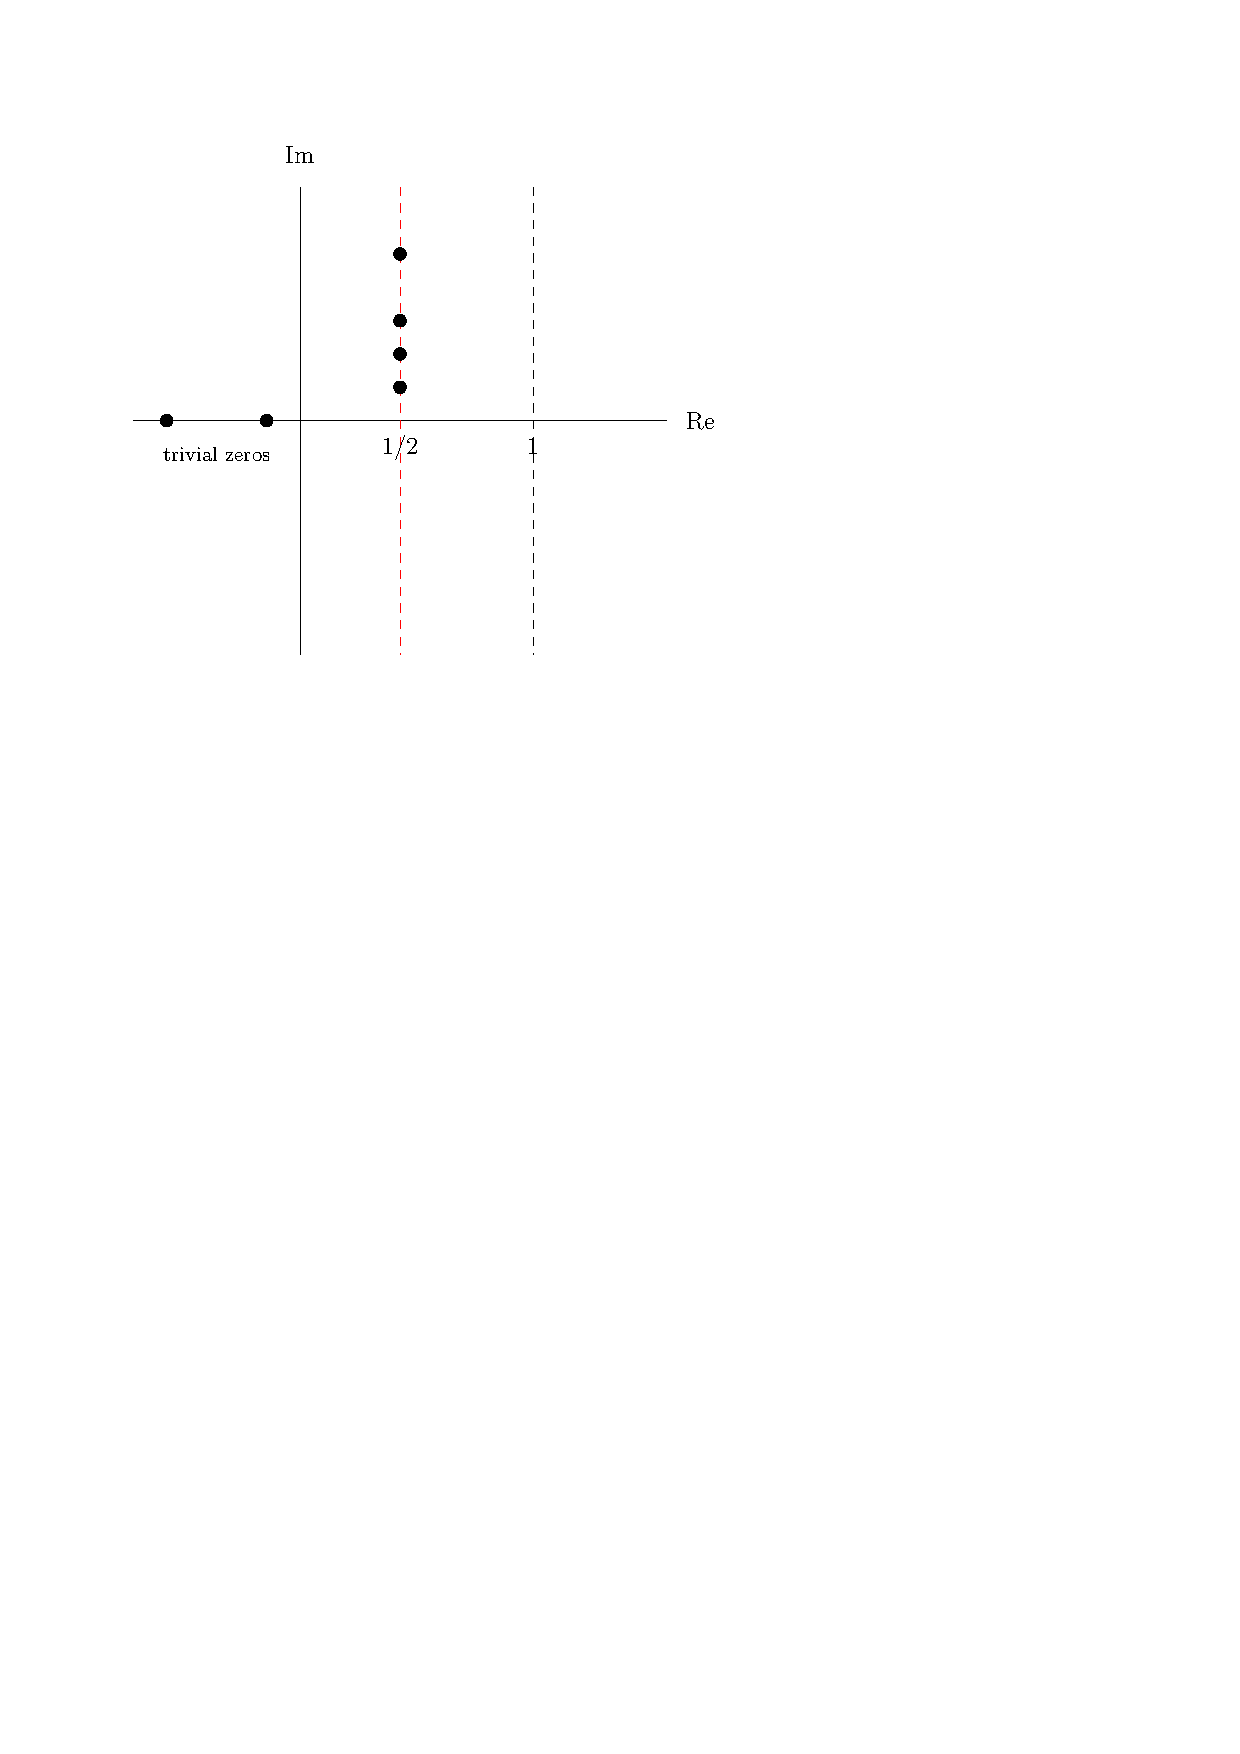
\includegraphics[width=.5\linewidth]{figures/riemann-hypothesis.pdf} 
    \caption{The non-trivial zeros of $\zeta(z)$ on a complex plane.}
    \label{fig:riemann-hypothesis}
\end{figure}

\end{document}